\chapter*{About this project}
\paragraph{Abstract}
This project is intended to be an project that can be used in an educational 
environment. During the Data Structures and Algorithms module we had in 2nd year,
short videos were shown to us showing various sorting algorithms being 
visualized. It is a web-based application written in ReactJS, a web framework 
for building user interfaces. The project allows users to visualize various
sorting algorithms, which could be helpful in an educational context.

\chapter{Introduction}
This chapter serves as an introduction to the project. In it, the various aspects
of the project are discussed and the main objectives of the project. Each of the 
chapters are briefly discussed as well, detailing what each contains and what is
discussed in each.

\section{Discussion of the dissertation}
Throughout this dissertation, the methodologies used throughout the development of the project, development tools, technology used and a review of each, the design of the system, and an evaluation of the system are discussed.

\begin{itemize}
    \item \textbf{Chapter 1 - Introduction} - Chapter 1 serves as the introduction to the project, discussing the aim of the project, an overview of sorting algorithms, the project itself, the objectives of the project, and the scope of the project.
    \item \textbf{Chapter 2 - Methodology} - Chapter 2 covers the various research and software methodologies employed throughout, meetings with the project supervisor. development tools used, source control, and types of testing carried out.
    \item \textbf{Chapter 3 - Technology Review} - Chapter 3 introduces each of the different technologies, tools, and languages used to develop the project itself.
    \item \textbf{Chapter 4 - System Design} - Chapter 4 discusses the design of the system and goes over each of the main components of the application.
    \item \textbf{Chapter 5 - System Evaluation} - Chapter 5 evaluates the system as a whole, analysing the various aspects of the project and further discusses the type of testing carried out.
    \item \textbf{Chapter 6} - Chapter 6 serves as the conclusion...
\end{itemize}

\section{Aim of the project}
The aim of this project is to create a web-based application that allows users to
visualise various different sorting algorithms, allow user authentication and 
upload visualisations to a database from which other users can view and compare
the performance. This project is intended to be used in an educational sense,
providing an interactive application where user's can actively choose a sorting
algorithm to visualise, save these visualisations to view them at a later point.

\section{Sorting Algorithms}
In computer science, a sorting algorithm is an algorithm that rearranges 
elements of a list in a certain order, according to a comparison operator on the
elements. The comparison operator is used to decide the new order of element in the respective data structure. The most frequently used orders are numerical order and lexicographical order. Efficient sorting is important for optimizing the efficiency of other algorithms (such as search and merge algorithms) that require input data to be in sorted lists. Sorting is also often useful for canonicalizing data and for producing human-readable output. More formally, the output of any sorting algorithm must satisfy two conditions:

\begin{enumerate}
    \item The output is in non-decreasing order (each element is no smaller than 
    the previous element according to the desired total order)
    \item The output is a permutation (a reordering, yet retaining all of the 
    original elements) of the input
\end{enumerate}

Furthermore, the input data is often stored in an array, which allows random 
access, rather than a list, which only allows sequential access; though many 
algorithms can be applied to either type of data after suitable modification.

\section{Discussion of the project}
The project is sorting algorithm visualiser that allows users to choose a sorting
algorithm to visualise. It also supports user authentication, where users can 
register and sign-in to save previous sorts. The project came about from viewing 
similar projects online and and an interest in finding out how such projects were
developed. The project also came about from developing something that could be 
used in an educational sense. In 2nd year of our course, we were enrolled in a 
Data Structures and Algorithms module from which we learned about various 
different algorithms, how they were performed, space time complexity, etc.

\newpage
\section{Objectives of the project}
There were several objectives I set out when first designing this project:

\begin{itemize}
    \item Create an application that can be used in an educational sense, which 
    can possibly be used for modules where students learn about data structures, 
    algorithms, space time complexity, etc.
    \item Create a web application that allows users to visualise several 
    different sorting algorithms.
    \item Allow users to register for an account and log in to save
    visualisations for later viewing.
    \item Allow users to upload their own 'data sets' to sort.
\end{itemize}

\section{Scope of the project}
\begin{center}
    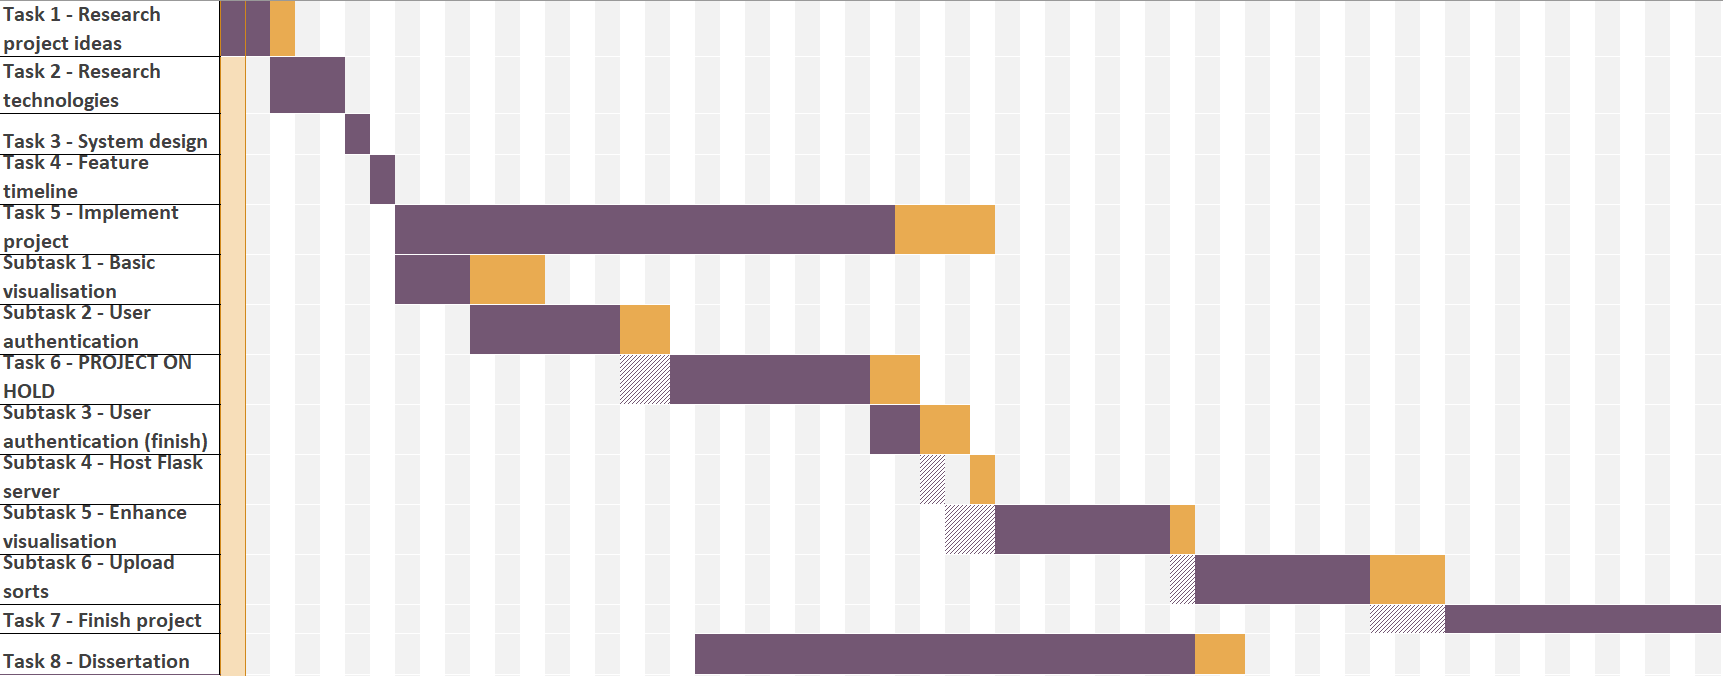
\includegraphics[scale=.3]{images/project_timeline} 
    \label{fig:project_timeline}
\end{center}

\subsection{Project Requirements}
\begin{center}
    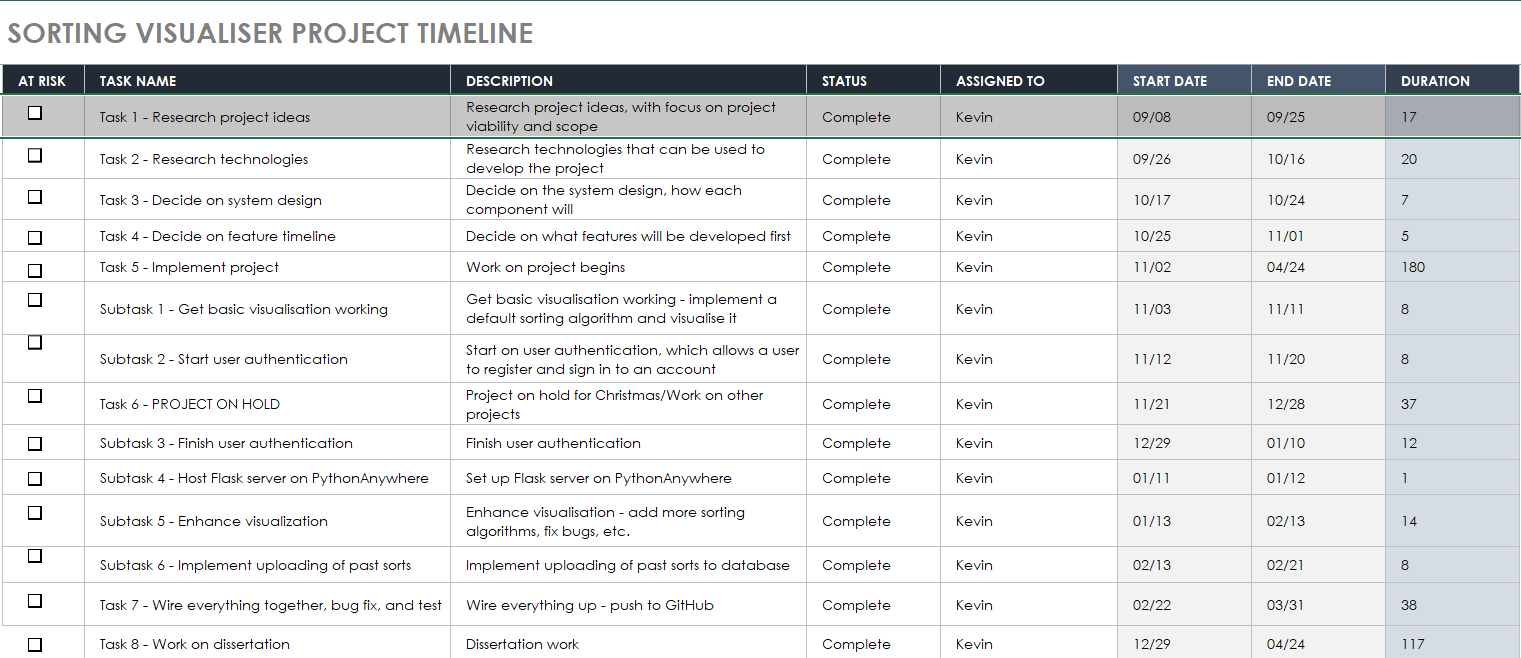
\includegraphics[width=16cm]{images/project_plan} 
    \label{fig:project_plan}
\end{center}
There were several project requirements that I set out when designing this
project. These can be seen in \ref{fig:project_timeline}. The functions and
features required were:

\begin{itemize}
    \item Visualisation of sorting algorithms
    \item Support of various sorting algorithms
    \item Upload of user created data sets
    \item User authentication
    \item Database support
\end{itemize}

\subsection{Process Requirements}

\subsection{Project Limitations}
As a whole, the application is primarily built to sort elements represented in a
numerical format. The limitations of the project would be the inability to sort 
elements represented in a numerical format, special characters, files, etc. In the context of an algorithms visualiser, while being able to sort items like letters, special characters, files, etc. could very well be viable, visualising such things mightn't be as suitable as visualising the sorting of numbers.